\label{section:Piece_level_Diff_Backtrack_Algorithm}

The CodeGlass server system needs to obtain commits that involve changes on the code piece selected by the user.
Such an algorithm needs to locate the portion in a past commit which best matches with the given code piece.
To make CodeGlass viable in realistic use, we have the following design considerations for the algorithm.

%       \begin{figure}[!t]
%         \centering
%             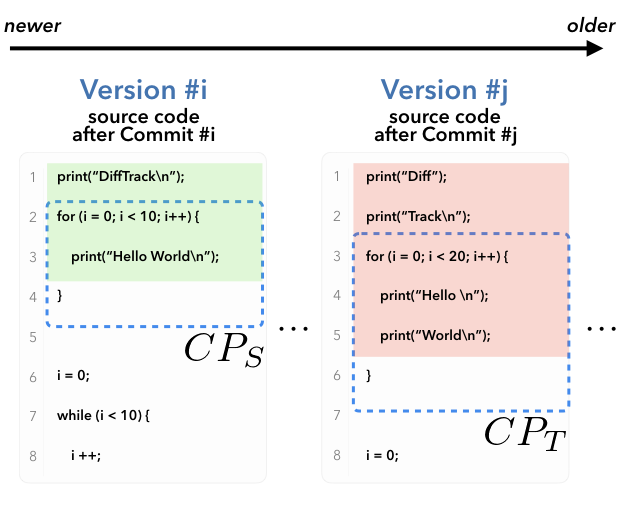
\includegraphics[width=0.9\columnwidth]{algorithm/limitation.png}
%             \caption{An example illustration of a source and true target code piece ($CP_{S}$ and $CP_{T}$). In this and following figures, red and green lines represent deleted and added lines between two versions (\#$i$ and \#$j$, $i>j$), respectively. A code piece in the newer version serves as $CP_S$ (lines in the broken frame in Version \#i). A backtrack algorithm estimates the location of $CP_{T}$ given $CP_{S}$, and runs iteratively with older commits. An estimated target code piece is denoted as $\widehat{CP_{T}}$. The ideal $\widehat{CP_{T}}$ is $CP_{T}$. This backtracking returns a series of commits associated with the code piece originally selected by the user.}

% 			\label{fig:CommitHistory}
%       \end{figure}
      
\begin{itemize}
\setlength{\parskip}{1mm}
\setlength{\leftskip}{7mm}
\setlength{\itemsep}{0cm}
\item[DC-1.] Accurately identify the location of a code piece in an older version even if changes occurred within it.
%\item[DC-2.] Run in real time regardless of the project scale and code length as well as the size of a code piece.
\item[DC-2.] Be compatible with any type of program-related files including style sheets and configuration files.
\item[DC-3.] Perform at a line-level granularity, from a single line to the entire file, to support unconstrained interaction.
\end{itemize}



      

Before explaining the details of our algorithm, we define a source and target code piece.
A source code piece ($CP_{S}$) means a code piece in a commit.
Using $CP_{S}$, the DiffTrack algorithm estimates a target code piece in an older commit.
We denote a true and estimated target code piece as $CP_{T}$ and $\widehat{CP_{T}}$, respectively.
Ideally, $\widehat{CP_{T}}$ is exactly the same set of lines of $CP_{T}$.
As the DiffTrack algorithm is executed iteratively, an additional subscript $i$ represents a code piece in the $i$-th version from the initial commit (i.e., $CP_{Si}$ is the source code piece in Version \#$i$).
We assume that the number of $CP_T$ is always one.

%The iteration occurs by using a target code piece as the source in the next step (i.e., $CP_{Sj} = \widehat{CP_{Ti}}$, $i>j \geq 1$).

\subsection{Limitations with git and git-blame commands}
\label{subsection:Limitations_with_git_commands}


%     \begin{figure}[tb]
%             \centering
%           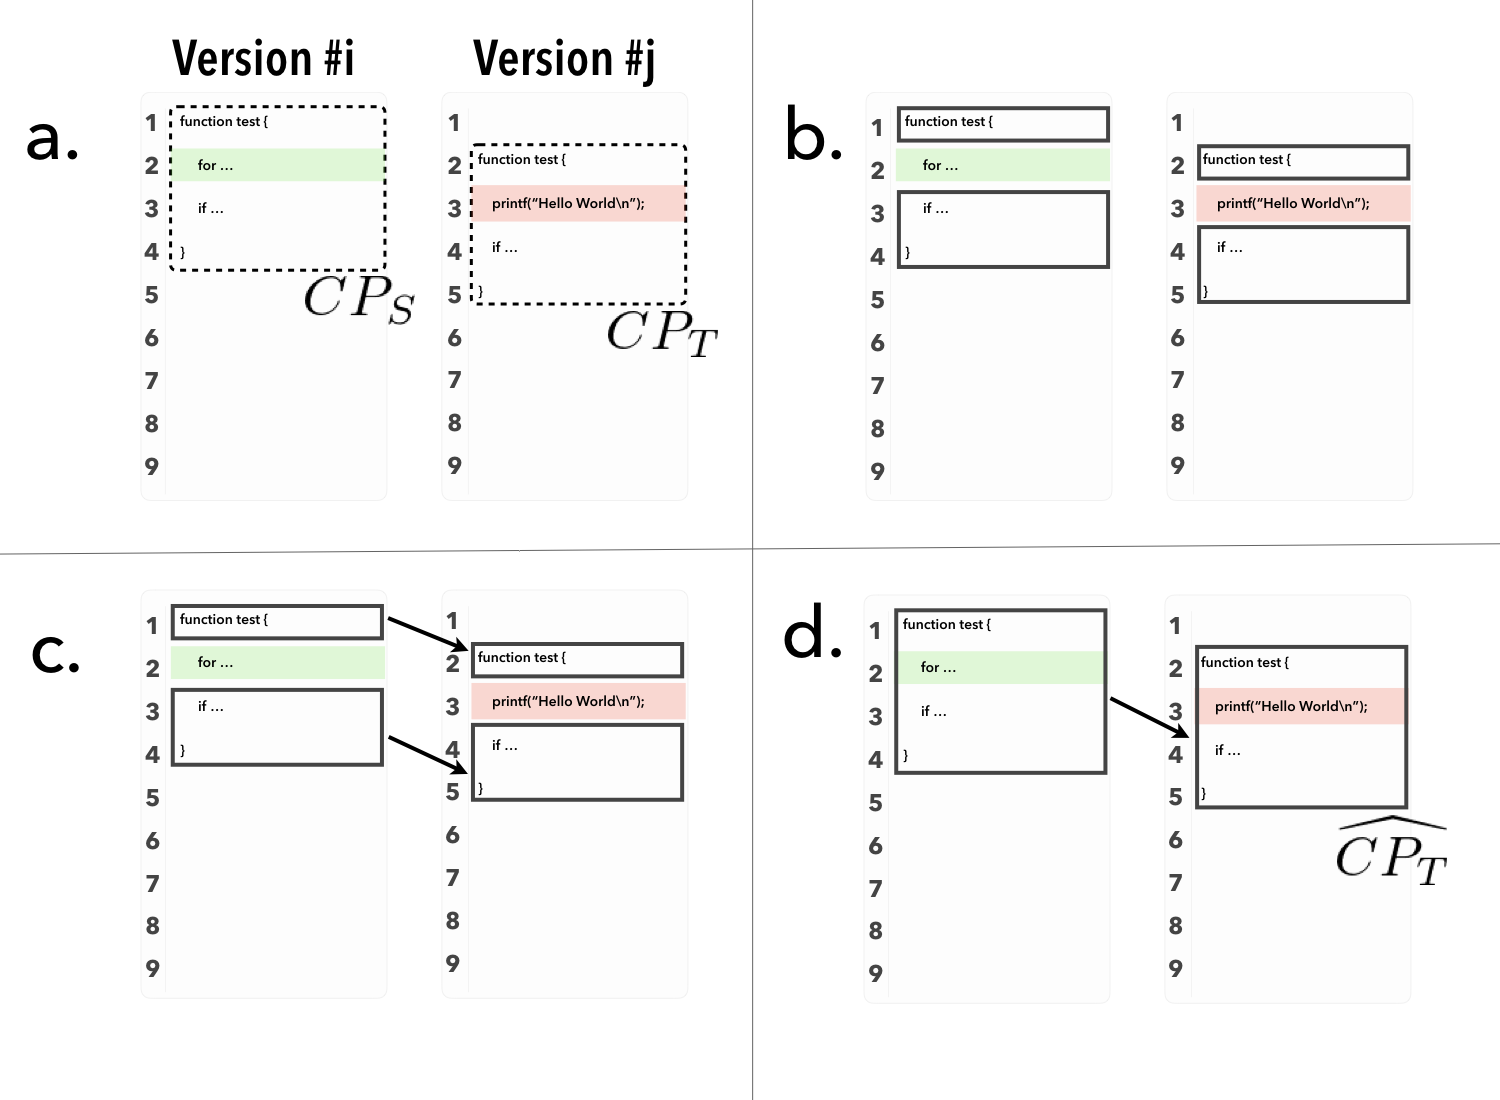
\includegraphics[width=1.0\columnwidth]{algorithm/Cases_001.png}
%           \caption{Case A: $CP_S$ includes unchanged lines that enclose the revised portion. (a) $CP_S$ and $CP_T$ are line 1--4 in the source commit and line 2--5 in the target commit, respectively. (b) The unchanged lines in $CP_S$ enclose the revised portion. (c) The unchanged lines serve as an anchor for search. (d) DiffTrack thus immediately determines line 2--5 as $\widehat{CP_T}$.}
%           \label{fig:caseA}
%     \vspace{-2mm}
%     \end{figure}


%     \begin{figure}
%       \centering
%         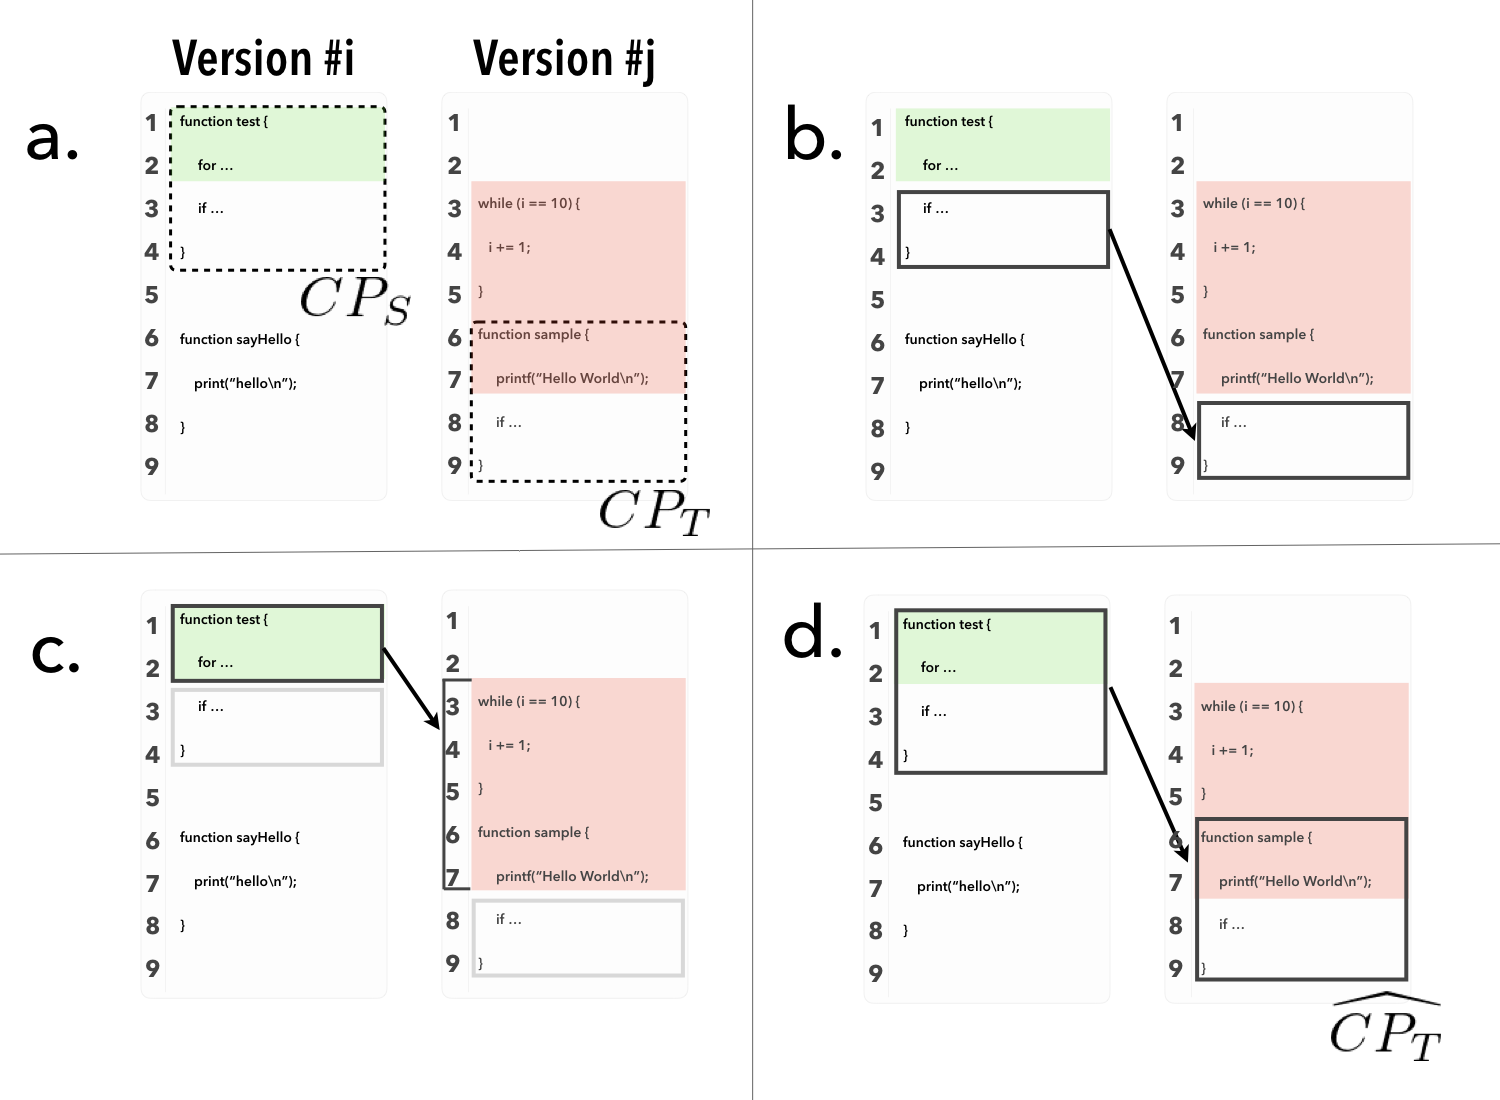
\includegraphics[width=1.0\columnwidth]{algorithm/Cases_002.png}
%         \caption{Case B: $CP_S$ includes unchanged lines that do not enclose the revised portion. (a) $CP_S$ and $CP_T$ are line 1--4 in the source commit and line 6--9 in the target commit, respectively. (b) DiffTrack first performs matching with the unchanged lines. (c) It removes unchanged lines (line 1 and 2) in the target commit from the search space. (d) It then performs fuzzy string search matching to identify lines most similar to the revised lines in the source commit. It finally determines line 6--9 $\widehat{CP_T}$.}~\label{fig:caseB}
%     \vspace{-5mm}
%     \end{figure}


Figure~\ref{fig:CommitHistory} shows an example of code changes between two versions (\#$i$ and \#$j$, $i > j$).
Suppose that our system needs to identify commits related to line 2--4 in Version \#$i$ to extract associated pull requests.
Thus, this portion is $CP_{Si}$~(the broken frame in Version \#$i$ in Figure~\ref{fig:CommitHistory}).
The git-blame command can point to the latest commit in which any part of $CP_{Si}$ was affected.
Thus, it is straightforward to find Commit \#$j$.
However, it provides \textit{only} the latest commit that contains changes in $CP_{Si}$.
This means that a system needs to find $CP_{Sj}$ (or $CP_{Ti}$) given $CP_{Si}$ to trace back to older commits and iteratively perform git-blame.
However, a diff log merely contains a set of line additions and deletions, which do not directly represent which revised lines are related to $CP_{Si}$.
In other words, git-blame cannot immediately provide the location of $CP_{Ti}$.
% In the example of Figure~\ref{fig:CommitHistory}, a system can only know that there are three lines of additions and five lines of deletions.
% But it is not immediately clear which revised lines are related to $CP_{Si}$, and we thus need a method to estimate the location of $CP_{Ti}$ (which also serves as $CP_{Sj}$ for further backtracking).

\subsection{Limitations with abstract syntax trees}

Another alternative approach is to use fine-grained source code change extraction methods~\cite{GumTree, Change_Distilling}.
These approaches can extract not only additions or deletions but also infer syntactic changes, such as updates or moves.
They use an abstract syntax tree (AST) to compute similarity between the two versions and extract syntactic changes.
%One example of such algorithms is Change Distiller developed by Fluri et al~\cite{Change_Distilling}.
%Falleri et al.'s GumTree~\cite{GumTree} further improve precisions on detecting code moves.
Although these algorithms are designed to compare multiple versions of an entire source code file, it is theoretically possible to implement them to perform matching of code pieces.


Nevertheless, we decided not to consider AST-based methods because they do not satisfy DC-2 and 3 in general.
As methods using abstract syntax trees require a parser, additional configuration is necessary for adaptation to different programming languages.
For example, GumTree~\cite{GumTree} is only compatible with C, Java, JavaScript, and Ruby as of April 2017.
Internal parsing can lead to large computational overhead for long code pieces.
In addition, a selected code piece should be syntactically correct, which also limits user experience.
We thus developed an algorithm called DiffTrack.

\subsection{DiffTrack Algorithm}

The DiffTrack algorithm can identify a set of commits that contain changes on a user-selected code piece.
It first finds the latest commit and version containing changes on the code piece by the git-blame command.
The algorithm then locates a portion of code in this version which is the most similar with the given code piece.
It then performs this operation iteratively by using the estimated portion of code as the next source code piece to trace back to even older versions.
For instance, in the example of Figure~\ref{fig:CommitHistory}, the estimated code piece (i.e., $\widehat{CP_{Ti}}$) given $CP_{Si}$ becomes $CP_{Sj}$.
The algorithm stops when it reaches to the oldest version or no reasonable $\widehat{CP_{T}}$ is found.
This process results in a set of commits containing changes on the code piece the user initially selects.
It finally extracts pull requests that include these commits and returns them to a client.
CodeGlass ultimately visualizes the pull requests in its interface.
In this section, we explain the behavior of DiffTrack with three cases in all of which $CP_{S}$ includes revisions.


\subsubsection{Case A: $CP_S$ includes unchanged lines that enclose the revised portion.}


$CP_S$ contains revised lines between the unchanged portions (i.e., line 2 in Version \#i in Figure~\ref{fig:caseA}).
In this case, the algorithm first uses the unchanged lines (line 1, 3, and 4) as an anchor to find $\widehat{CP_T}$.
In addition, only changed lines should be included between the unchanged portions.
The algorithm, therefore, immediately identifies $\widehat{CP_T}$ as the unchanged portions and changed lines in-between (i.e., line 2--5 in Version \#$j$).

\subsubsection{Case B: $CP_S$ includes unchanged lines that do not enclose the revised portion.}

%     \begin{figure}[tbp]
%             \centering
%           \includegraphics[clip, width=8cm]{algorithm/CaseB.png}
%           \caption{An example of case B (where $CP_S$ includes unchanged lines that do not enclose the revised portion).
%           $CP_S$ and $CP_T$ are from line 1 to 4 in the source commit and from line 6 to 9 in the target commit, respectively.~(a)
%           The algorithm first perform matching with the unchanged lines.
%           In this example, codes from line 3 to 4 in the source commit matches with counterparts from line 8 to 9 in the target commit.~(b)
%           The algorithm removed unchanged lines from the target commit (i.e., line from 1 to 2 in the target commit) to prune the search space.~(c)
%           It then performs fuzzy string search matching to identify codes most similar to the revised lines~(i.e., line 1 and 2 in the source commit).
%           The algorithm finally determines from line 6 to 9 in the target commit as $CP_T$.~(d)
%           }
%           \label{fig:caseB}
%     \end{figure}
    

$CP_S$ contains unchanged lines, but the revised portion is not enclosed.
Figure \ref{fig:caseB} presents such an example where the first half has been revised while the other stays unchanged.
   
Similar to the previous case, the algorithm first performs matching with the unchanged lines.
This matching result narrows down the possible lines for $\widehat{CP_T}$ (above line 7 in this example).
The algorithm further reduces the search space by removing remaining unchanged lines because it can assume that the rest of $\widehat{CP_T}$ should be revised lines.
In this example, line 1 and 2 are unchanged, and thus they are removed from the search.
The algorithm then performs fuzzy string matching between the revisions (explained in detail later), and identifies the set of lines with the highest similarity score (line 6 and 7 in this example).
DiffTrack determines line 6--9 as $\widehat{CP_T}$.


\subsubsection{Case C: $CP_S$ does not include unchanged lines.}

%     \begin{figure}[tbp]
%             \centering
%           \includegraphics[clip, width=8cm]{algorithm/CaseC.png}
%           \caption{An example of case C (where $CP_S$ does not include unchanged lines).
%           $CP_S$ and $CP_T$ are from line 1 to 3 in the source commit and from line 5 to 7 in the target commit, respectively.~(a)
%           The algorithm first removes all unchanged lines from the target commit.~(b)
%            It then performs fuzzy string matching on all possible string chunks, and finds the most similar match.~(c)
%            The algorithm finally determines codes from line 5 to 7 in the target commit as $CP_T$.~(d)}
%           \label{fig:caseC}
%     \end{figure}
    
% \begin{figure}
%     \centering
%       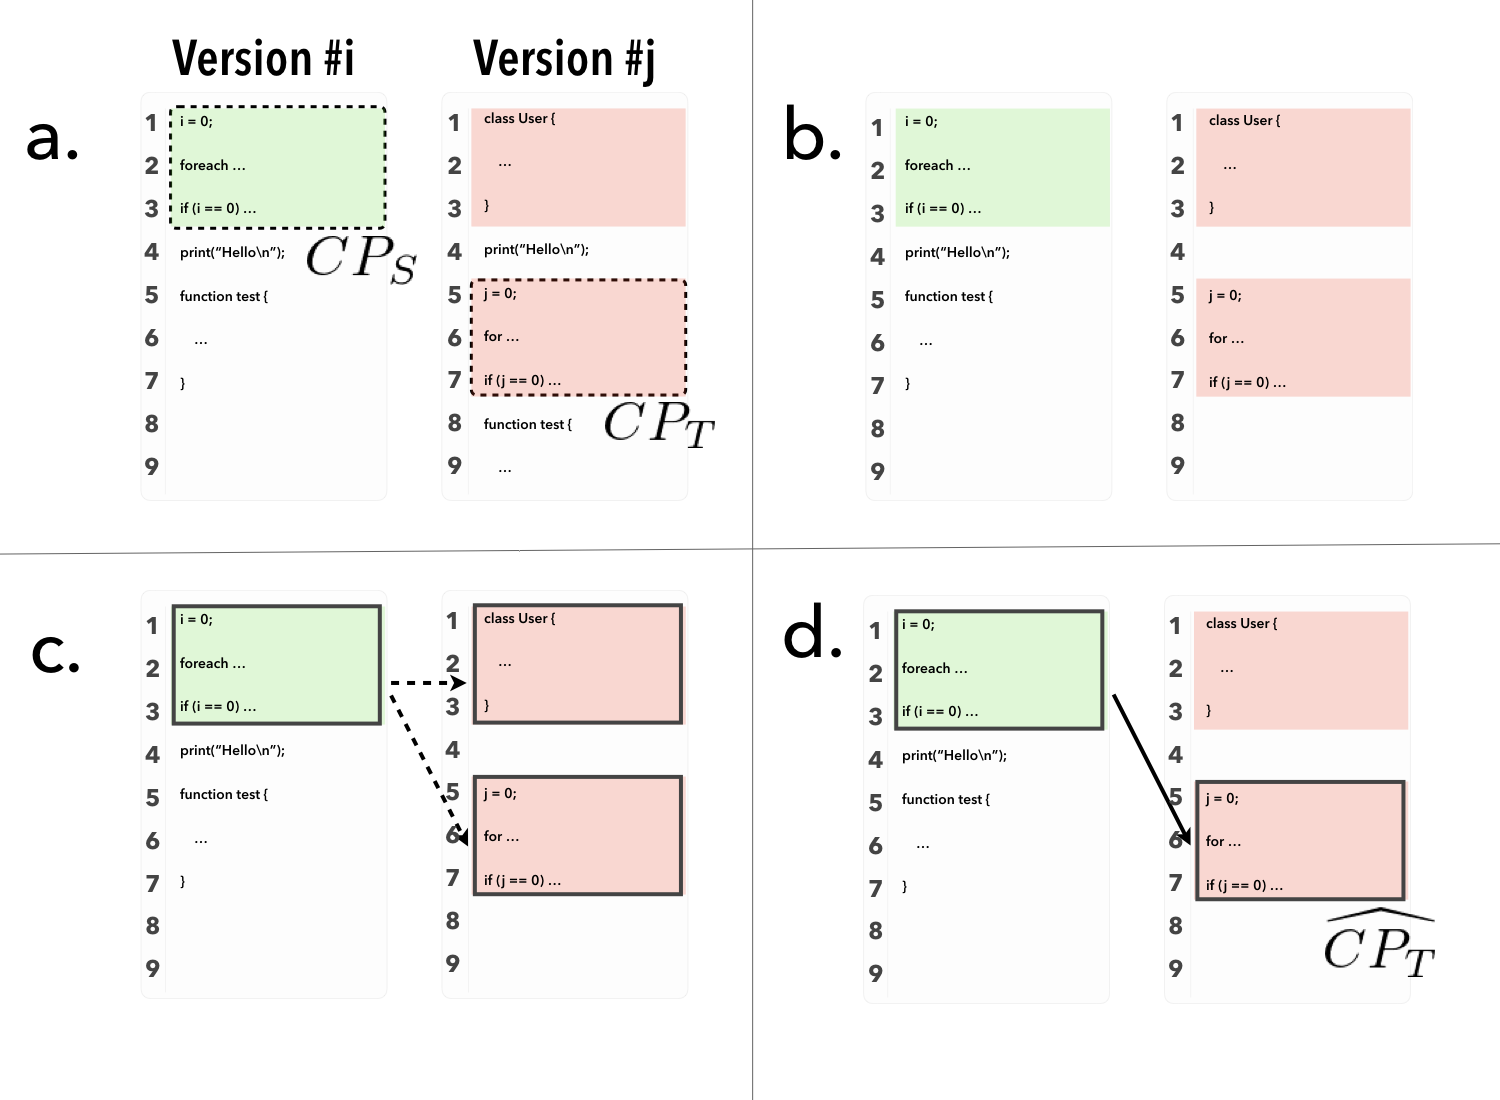
\includegraphics[width=1.0\columnwidth]{algorithm/Cases_003.png}
%       \caption{Case C: $CP_S$ does not include unchanged lines (a) $CP_S$ and $CP_T$ are line 1--3 in the source commit and from line 5--7 in the target commit, respectively. (b) DiffTrack first removes all unchanged lines from the search. (c) It then performs fuzzy string matching on all possible string chunks, and finds the most similar match. (d) DiffTrack finally determines line 5--7 in the target commit as $\widehat{CP_T}$.}~\label{fig:caseC}
%     \vspace{-5mm}
%     \end{figure}



The two example above demonstrates that unchanged lines in $CP_S$ serve as a useful anchor for determining $\widehat{CP_T}$.
However, $CP_S$ may not contain any unchanged line as illustrated in Figure \ref{fig:caseC}.
In this case, DiffTrack first removes all unchanged lines from the search.
This would result in string chunks (i.e., sets of consecutive code lines) as shown in Figure \ref{fig:caseC}.
The algorithm then performs fuzzy string matching on all chunks and sub-chunks, and finds the most similar match.

\subsection{Fuzzy String Matching}
The DiffTrack algorithm performs fuzzy string matching to identify a code piece most similar to $CP_S$ in the target commit.
It uses a variant of the Levenshtein distance as a cost function.
The Levenshtein distance is defined as the minimum number of character operations that are necessary to convert a string to another.
Character operations include additions, deletions and substitutions.
In our fuzzy string matching, we calculate the distance on a word basis with different weights on change operations (1, 1, and 2 for additions, deletions and substitutions, respectively).
For example, the cost of a conversion from ``int x = 1 + 2;'' to ``float x = 1.0;'' is 6 because there are 2 deletions and 2 substitutions.
Our fuzzy matching also considers the length of $CP_S$ and a possible target code piece ($cp$).
The DiffTrack algorithm thus uses the following similarity score to find possible a target code piece:

% \koji{}{Maybe explain why we use word-based similarity rather than char-based?}

\begin{equation}
Sim(cp) = \frac{wp(CP_S) + wp(cp) - LDw(CP_S,\, cp)}{wp(CP_S) + wp(cp)},
\end{equation}

where $wp(x)$ is the word count in text $x$, and $LDw$ is a word-level Levenshtein distance.
$Sim(cp)$ takes a value between 0 and 1, representing that higher is more similar.
We use a brute-force approach to find a code piece with the highest similarity score.

\subsection{Graceful Code Piece Matching}

    
DiffTrack determines $\widehat{CP_T}$ as a code piece with the highest similarity score under an assumption that the number of $CP_T$ is always one.
We set a threshold (Definitive Matching Threshold, DMT) to determine if there exists any possible target code piece with strong belief.
But, the fuzzy string matching method may still fail to determine a clear target code piece when changes are substantial.
To allow graceful matching, we set another threshold (Candidate Matching Threshold, CMT).
The graceful matching creates a list of likely target code pieces instead of simply stopping search.

To determine appropriate values for these threshold, we created a dataset containing 49 commits (i.e., 49 pairs of two versions) in Chart.js.
This dataset deliberately contained only revisions that included refactoring.
Estimating a match in these revisions is presumably difficult with DiffTrack.
In each pair, we manually labeled $CP_S$ and $CP_T$.
We also chose a code piece which was a disjoint set of $CP_T$ and exhibited the highest similarity score as the most similar incorrect match ($IM$).

Figure~\ref{fig:histogram_sim} summarizes the occurrences of similarity scores of $CP_T$ (in blue) and $IM$ (in pale orange).
This histogram clearly illustrates that similarity scores of $IM$ are below 0.65.
It also shows that the scores of $CP_T$ are above 0.45.
We, therefore, determined DMT and CMT to be 0.65 and 0.4, respectively.

In Case C, the default DiffTrack algorithm stops backtracking when it finds no code piece with a higher value than DMT.
With graceful matching, the algorithm additionally searches all possible code pieces with the similarity scores above CMT after backtracking.
In order to capture cases in which a code piece was moved from a file to another, the graceful matching process checks all files in a repository that contain any revision. 
The algorithm first sorts them by the similarity scores in the descending order and initializes a list for candidate target code pieces.
For each possible code piece, the algorithm checks if it is mutually exclusive with all lines in the current candidate list.
If true, the algorithm adds that code piece to the candidate list.
All code pieces in this candidate list are finally shown to the user in the interface ((2) in Figure~\ref{fig:WebInterface}a).

DiffTrack does not use any threshold value for Case B.
It regards a code piece with the highest similarity score as $\widehat{CP_T}$.

%     \begin{figure}
%       \centering
%         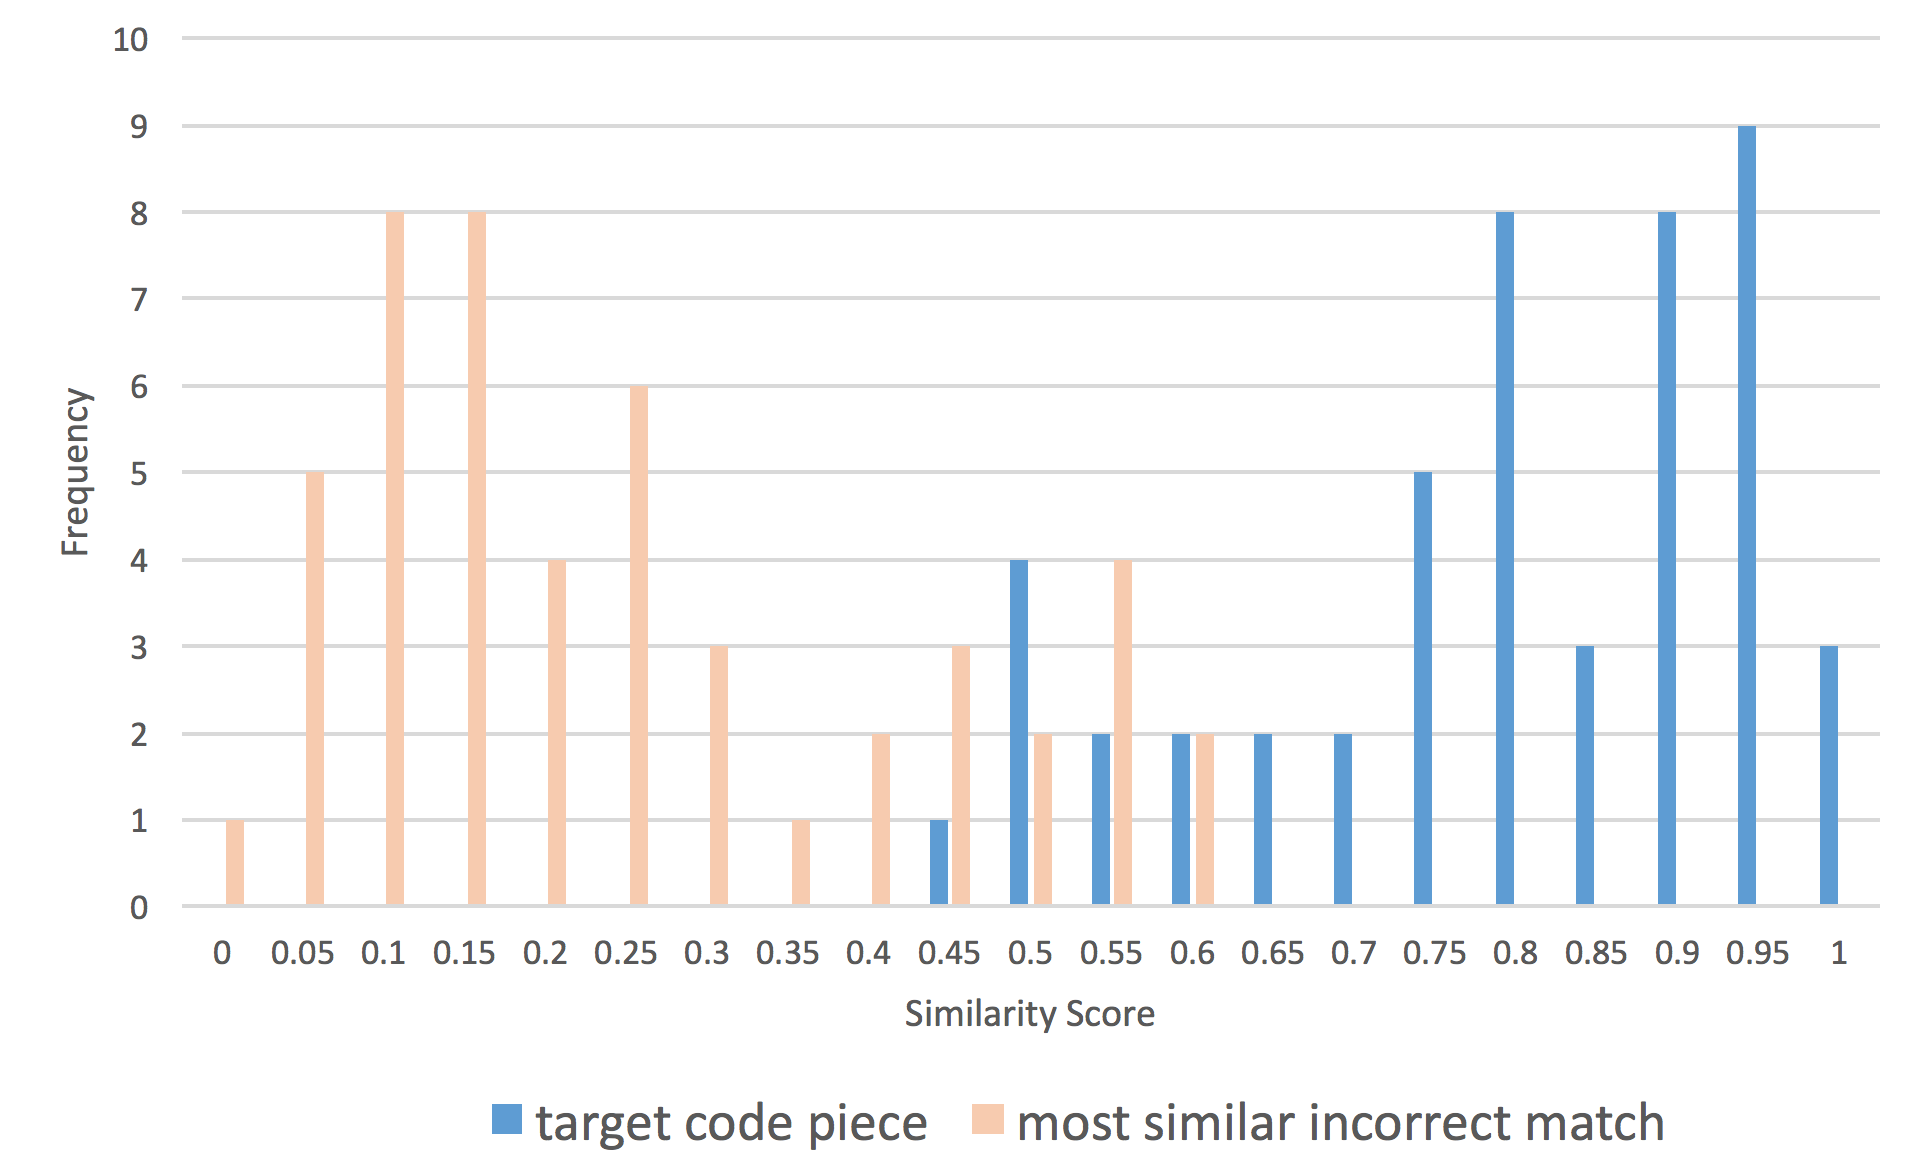
\includegraphics[width=1.0\columnwidth]{algorithm/histogram_sim.png}
%         \caption{The occurrence distributions of similarity scores of $CP_T$ (in blue) and most similar incorrect matches ($IM$, in pale orange).}~\label{fig:histogram_sim}
%     \end{figure}


